\documentclass[draft]{agujournal2019}


%\journal{jpo}
\usepackage{graphicx}
\usepackage{mathtools}
\usepackage{mathrsfs}
\usepackage{amssymb}
\usepackage{amsmath}
\usepackage{amsfonts}
\usepackage{bm}
\usepackage{svg}
\newcommand{\vu}{\bm{u}}
\newcommand{\vv}{\bm{v}}
\newcommand{\vx}{\bm{x}}
\newcommand{\vk}{\bm{k}}
\newcommand{\vtau}{\bm{\tau}}
\newcommand{\pt} {\frac{\partial}{\partial t}}
\newcommand{\n}{\nabla}
\newcommand{\beq}{\begin{equation}}
\newcommand{\eeq}{\end{equation}}
\newcommand{\rf}{\ref}
\newcommand{\lb}{\label}
\newcommand{\hu}{\hat{u}}
\newcommand{\hv}{\hat{v}}
\newcommand{\hw}{\hat{w}}
\newcommand{\hK}{\hat{K}}
\newcommand{\hp}{h^{\#}}
\newcommand{\Wp}{w^{\#}}
\newcommand{\pp}{p^{\#}}
\newcommand{\bp}{b^{\#}}
\newcommand{\pz}{\frac{\partial}{\partial z}}
\newcommand{\vp}{\bm{\xi}}
\newcommand{\hnu}{\hat{\nu}}
\newcommand{\Sb}{\overline{\sigma}}
\newcommand{\hk}{\widehat{K"}}
\newcommand{\hh}{\hat{h}}
\newcommand{\md}{\frac{d}{dt}}
\newcommand{\vb}{\bm{\beta}}
\newcommand{\vg}{\bm{\gamma}}
\newcommand{\T}   {\scriptstyle \mathsf{T}}
\newcommand{\mat} [1]{\pmb{\mathsf{#1}}}
%%%%% Drew TeX  %%%%%%
\newcommand{\bu}{\bm{u}}
\newcommand{\bv}{\bm{v}}
\newcommand{\part} [2]{\frac{\partial{#1}}{\partial{#2}}}
%%%%% End Drew TeX  %%%%%%
\journalname{Journal of Advances in Modeling Earth Systems (JAMES)}

\begin{document}
%%%%%%%%%%%%%%%%%%%%%%%%%%%%%%%%%%%%%%%%%%%%%%%
%  TITLE
%
% (A title should be specific, informative, and brief. Use
% abbreviations only if they are defined in the abstract. Titles that
% start with general keywords then specific terms are optimized in
% searches)
%
%%%%%%%%%%%%%%%%%%%%%%%%%%%%%%%%%%%%%%%%%%%%%%%

\title{Spectra in Irregular Domains}

%%%%%%%%%%%%%%%%%%%%%%%%%%%%%%%%%%%%%%%%%%%%%%%
%
%  AUTHORS AND AFFILIATIONS
%
%%%%%%%%%%%%%%%%%%%%%%%%%%%%%%%%%%%%%%%%%%%%%%%

% Authors are individuals who have significantly contributed to the
% research and preparation of the article. Group authors are allowed, if
% each author in the group is separately identified in an appendix.)

% List authors by first name or initial followed by last name and
% separated by commas. Use \affil{} to number affiliations, and
% \thanks{} for author notes.
% Additional author notes should be indicated with \thanks{} (for
% example, for current addresses).

% Example: \authors{A. B. Author\affil{1}\thanks{Current address, Antartica}, B. C. Author\affil{2,3}, and D. E.
% Author\affil{3,4}\thanks{Also funded by Monsanto.}}

\authors{Joseph Schoonover\affil{1}, William K. Dewar\affil{2}, Andrew Poje\affil{3}, Nicolas Wienders, Garrett Byrd\affil{1}, Siddhartha Bishnu\affil{4}}


\affiliation{1}{Fluid Numerics LLC, Hickory, NC, USA}
\affiliation{2}{Florida State University, Tallahassee, FL, USA}
\affiliation{3}{City University of New York, New York, NY, USA}
\affiliation{4}{Department of Earth Sciences, University of Cambridge, United Kingdom}

% Corresponding author mailing address and e-mail address:
\correspondingauthor{Joseph Schoonover}{joe@fluidnumerics.com}



%%%%%%%%%%%%%%%%%%%%%%%%%%%%%%%%%%%%%%%%%%%%%%%
% KEY POINTS
%%%%%%%%%%%%%%%%%%%%%%%%%%%%%%%%%%%%%%%%%%%%%%%
%  List up to three key points (at least one is required)
%  Key Points summarize the main points and conclusions of the article
%  Each must be 140 characters or fewer with no special characters or punctuation and must be complete sentences

% Example:
% \begin{keypoints}
% \item	List up to three key points (at least one is required)
% \item	Key Points summarize the main points and conclusions of the article
% \item	Each must be 140 characters or fewer with no special characters or punctuation and must be complete sentences
% \end{keypoints}

\begin{keypoints}
\item enter point 1 here
\item enter point 2 here
\item enter point 3 here
\end{keypoints}

%%%%%%%%%%%%%%%%%%%%%%%%%%%%%%%%%%%%%%%%%%%%%%%
%
%  ABSTRACT and PLAIN LANGUAGE SUMMARY
%
% A good Abstract will begin with a short description of the problem
% being addressed, briefly describe the new data or analyses, then
% briefly states the main conclusion(s) and how they are supported and
% uncertainties.

% The Plain Language Summary should be written for a broad audience,
% including journalists and the science-interested public, that will not have 
% a background in your field.
%
% A Plain Language Summary is required in GRL, JGR: Planets, JGR: Biogeosciences,
% JGR: Oceans, G-Cubed, Reviews of Geophysics, and JAMES.
% see http://sharingscience.agu.org/creating-plain-language-summary/)
%
%%%%%%%%%%%%%%%%%%%%%%%%%%%%%%%%%%%%%%%%%%%%%%%



\begin{abstract}
Ocean models in realistic settings are now standard. We consider in this paper methods for their dynamic analysis, particularly calculation of their kinetic energy spatial spectra. Realistic models pose difficulties when classical methods are applied, due to spatial inhomogeneity and complex geometries. Here, we leverage the Helmholtz decomposition of a vector field to decompose a 2-D velocity field into its rotational and divergent parts, represented by a streamfunction and velocity potential. The classical problem of Helmholtz decompositions, that the associated boundary conditions are not unique, is sidestepped by arguing appropriate conditions on both cast the kinetic energy of the domain solely in terms of the rotational and divergent contributions. Further exploiting the properties of the Helmholtz equation subject to homogenous boundary conditions allows for complete representation of the streamfunction and velocity potential in terms of orthonormal basis functions. Ultimately this leads to an exact representation of the domain kinetic energy in terms of the projections of the velocity fields on those functions and their eigenvalues, without the need for any windowing or interpolation. This is a decomposition equivalent to Parseval’s equality and permits the interpretation of the results as energy densities in eigenvalue space. Parallels between Fourier analysis and this more general approach argue that the amplitudes plotted against the eigenvalues plays the same role as Fourier based spectra. The generality of the analysis allows it to be applied to open domains, with inflow and outflow, and irregular domains with coastlines and islands. We develop a numerical discretization and a methodology for calculating the eigenfunctions and eigenvalues in complex domains on an Arakawa C-Grid and demonstrate the calculation of spectra on GPU accelerated hardware. We apply the technique to some idealized quasi-geostrophic simulations in closed domains to demonstrate capabilities in coping with irregular outer boundaries. We conclude with a discussion about applications to regional problems with open boundaries, geometries with islands, and models that support both rotational and divergent modes.
\end{abstract}

\section{Introduction}
In the last decades, there has been a proliferation of realistic ocean models, involving full basin geometry and forced by an array of reanalysis atmospheric products. These can be global or regional in scope, and certainly appear to be skilled at reproducing realistic looking ocean states. As such, it is of interest to analyze their dynamics in detail, with a common focus being wavenumber spectra of ocean kinetic energy.


At the moment, there are at least two issues with the computation of spatial spectra in such models. First, ocean domains are highly irregular in space, including such complications as interior islands and complex coastlines. Classical spectral techniques are almost solely based on Fourier analysis and to apply them to such regions involves interpolation over interior land regions and data manipulation, such as windowing, to bring the domain edges into consistency with the Fourier basis. A second problem is the ocean environment is highly inhomogeneous, implying that spatial spectra computed over a large domain mix together regions of different dynamics. An example would be the North Atlantic ocean, where a subtropical domain based spatial spectra would involve the separated Gulf Stream and the quiescent interior. It is thus unclear how representative any emerging spectrum is to subregions of the domain.

%\cite{uchida2025,uchida2022}
In view of this latter point, some recent analyses have resorted to analyzing smaller subdomains of a gyre with the idea that the associated spectra are more representative of subareas within the gyre. While recognizing the value of these approaches, the naturally occurring inflows and outflows at the domain edges are generally not periodic and require processing to force the data into forms amenable to Fourier analysis. In the above settings, a wedge is driven between the original data itself and the end state product. In the best case, this introduces artificialities into the data that obscure the meaning of the resulting spectra. In the worst case, it renders the spectral estimates invalid. We address both of these issues in this paper, the goals of which are twofold. First, we present an analysis method that avoids the above pitfalls and can lay claim to the spectral representation of kinetic energy in irregular and open domains at the same level of validity normally assigned to Fourier spectra. And, second, we apply and discuss the method in test settings that illustrate the flexibility in coping with irregular boundaries.

Most realistic general circulation modeling is based in the primitive equations, which incorporate assumptions of incompressibility and small aspect ratio. The momentum equations of this set are
\begin{subequations}
    \begin{align}
        u_t + uu_x + vu_y + wu_z - fv &= -p_x \\
        v_t + uv_x + vv_y + wv_z + fu &= -p_y
    \end{align}
\end{subequations}
where we ignore viscous terms, $u$ and $v$ are the $x$ and $y$ components of the velocity field, $w$ the vertical velocity, $f$ the Coriolis parameter, and $p$ the hydrostatic pressure. A kinetic energy equation is formed by vector multiplying the above equations by horizontal velocity, which identifies
\begin{equation}
    K = \frac{u^2 + v^2}{2}
\end{equation}
as the kinetic energy. It is frequently of interest to compute the wavenumber spectrum of this quantity. In any practical problem, the domain, A, over which velocity is known is finite, so traditionally Fourier series are employed. Defining $a_{n,m}$ , $b_{n,m}$ as the complex Fourier coefficients obtained via
\begin{subequations}
    \begin{align}
        a_{n,m} &= \int_A u e^{2 \pi i(nx/L_x + my/L_y)} dA \\
        b_{n,m} &= \int_A v e^{2 \pi i(nx/L_x + my/L_y)} dA
    \end{align}
\end{subequations}
where $L_x$ , $L_y$ are the zonal and meridional domain widths and $n, m$ are integers. Note that inherent in this is the assumption that the domain is relatively simple and rectangular. Fourier based spectra have the property that they obey Parseval’s equality, namely
\begin{equation}
    \int_A u^2 + v^2 dA = \sum_{n=-\infty}^{\infty}\sum_{m=-\infty}^{\infty}\left( a_{n,m}^2 + b_{n,m}^2\right)
\end{equation}
which permits the identification of the Fourier amplitude as an energy density in wavenumber space. 

While it is possible to perform this exercise in the presence of any velocity field, non-periodicity, inherent in any realistic velocity field, yields very slowly decaying spectral values at large wavenumbers. In essence, this arises because the data is inconsistent with the boundary conditions for which Fourier series were developed. Strategies for minimizing this effect, such as windowing the data, are frequently employed to bring the filtered data into a form consistent with the Fourier basis. In addition, if the domain also houses interior islands, it is necessary to interpolate over them to provide the data required to compute the coefficients. Last, most realistic domains are not rectangular, so some degree of data manipulation is required for coefficients to be calculated. A view that we adopt in this paper is that all these machinations, which are potentially harmful to the results, reflect attempting to use an ill-suited basis for the expansion, and that this can be improved upon.

We point out for reference that Fourier modes are complex exponentials, and as such satisfy the Sturm-Liouville eigenvalue problem
\begin{subequations}
    \begin{align}
        \nabla^2 f_{n,m} &= -\lambda_{n,m}^2 f_{n,m} \\
        f_{n,m}(0,y) &= f_{n,m}(L_x,y) \\
        f_{n,m}(x,0) &= f_{n,m}(x,L_y)
    \end{align} \label{eq:fourier basis problem}
\end{subequations}
where
\begin{equation}
    \lambda_{n,m}^2 = 4\pi^2((n/L_x)^2 + (m/L_y)^2) \label{eq:fourier eigenvalues}
\end{equation}
are the eigenvalues. In essence, the Fourier modes are basis functions generated from a Sturm-Liouville eigenvalue problem, where the boundary conditions are periodic. Our approach is to instead generate basis functions that satisfy boundary conditions that are consistent with regional velocity fields in irregular domains. This is done by expressing vector fields as a Helmholz decomposition and developing field equations and boundary conditions for the Helmholz potentials. In deriving these equations, we are able to show that a consistent set of basis functions come from Sturm-Liouville problems where the field operator is the Laplacian operator and the boundary conditions are homogeneous Dirichlet or homogenous Neumann. 

In section \ref{sec:Helmholz decomposition} we derive the equations and boundary conditions for the Helmholz potentials and discuss the expression for kinetic energy under the Helmholz decomposition. In section \ref{sec:Spectral decomposition} we present the Sturm-Liouville problems for the Dirichlet and Neumann modes and derive some of their properties. In section \ref{sec:Greens expansion} we show how we can use Green's solution to Poisson's equation to express the Helmholz potentials as a superposition the Dirichlet and Neumann modes while accounting for the possibility of open boundary conditions. In section \ref{sec:Calculating spectra} we present a proof of satisfaction of Parseval's equality for this decomposition, show an expression for energy density and present an argument for relating the eigenvalues to the length scales associated with the energy density. In section \ref{sec:Discretization}, we describe how we generate the Neumann and Dirichlet eigenpairs numerically, using a finite volume discretization on an Arakawa-C grid and matrix free methods for an efficient algorithm.

\section{Theory}
\subsection{Helmholtz decomposition} \label{sec:Helmholz decomposition}
Suppose we have a field of velocity data inside some domain with boundary velocities of any value. It is known that any vector field can be written via a Helmholtz decomposition into rotational and divergent parts. Here, we consider a two-dimensional vector field, representative of a fluid velocity field, 
\begin{equation}
    \vec{u} = (u,v) = (u_r + u_d, v_r + v_d) = (-\psi_y + \chi_x, \psi_x + \chi_y) \label{eq:helmholz decomposition}
\end{equation}
where $(u,v)$ are zonal and meridional velocity components, $\psi$ denotes the rotational potential and $\chi$ the divergent potential. Calculating the vorticity from equation \eqref{eq:helmholz decomposition} gives an equation for $\psi$ 
\begin{equation}
    \nabla^2 \psi = \nabla \cdot ( \hat{z} \times \vec{u} ) = \zeta
\end{equation}
and the divergence gives an equation for $\chi$,
\begin{equation}
    \nabla^2 \chi = \nabla \cdot \vec{u} = d.
\end{equation}
Given appropriate boundary conditions, these equations can be solved for $\psi$ and $\chi$.

A classical problem with a Helmholtz decomposition is its non-uniqueness due to the indeterminate boundary conditions on the rotational and divergent velocity contributions, as boundary conditions apply to the total velocity and not to each component individually. However, as pointed out by \cite{Fox-Kemper2003}, this non-uniquess in decomposition may still result in unique integral measures. Consider the form of kinetic energy written in rotational and divergent components,
\begin{equation}
    2K = u_r^2 + 2u_ru_d + u_d^2 +v_r^2 + 2v_rv_d + v_d^2
\end{equation}
and integrated over a domain $A$. Employing the Helmholtz decomposition, this becomes
\begin{equation}
    \int_A u^2 + v^2 \hspace{1mm}dA = \int_A (\nabla \psi \cdot \nabla \psi + \nabla \chi \cdot \nabla \chi + 2\nabla\psi \times \nabla \chi) \hspace{1mm}dA
\end{equation}
The last term, involving the cross product of $\nabla \chi$ and $\nabla \psi$, can be written in either of two forms
\begin{equation}
    \int_A \nabla\psi \times \nabla \chi \hspace{1mm}dA = \oint_{\partial A} \psi \nabla \chi \cdot \hat{t} dl = - \oint_{\partial A} \chi \nabla \psi \cdot \hat{t} dl \label{eq:energy cross product term}
\end{equation}
where $\hat{n}$ is the unit outward pointing normal vector at the domain edge $\partial A$ and $\hat{t}$ is the unit tangent vector pointing along the domain edge and oriented $90^\circ$  counterclockwise from $\hat{n}$. Determining a value for this term in the kinetic energy depends on the boundary conditions that are applied to $\psi$ and $\chi$.

The known velocities on the boundaries provide two constraints, one for each of the normal and tangential components of the flow,
\begin{subequations}
    \begin{align}
        \vec{u}\cdot \hat{n} &= \nabla \chi \cdot \hat{n} - \nabla \psi \cdot \hat{t} \\
        \vec{u} \cdot \hat{t} &= \nabla \chi \cdot \hat{t} + \nabla \psi \cdot \hat{n}
    \end{align}
\end{subequations}
These two equations provide a number of possible boundary conditions for $\chi$ and $\psi$, and a choice for a boundary condition for one of the potentials determines a necessary boundary condition for the other. As pointed out by \cite{Fox-Kemper2003}, it is sufficient to extract boundary conditions from one of these.  For example, choosing 
\begin{equation}
    \vec{u} \cdot \hat{n}|_{\partial A} = \nabla \chi \cdot \hat{n}|_{\partial A} \label{eq:normal velocity matching}
\end{equation}
implies that
\begin{equation}
    \nabla \psi \cdot \hat{t} |_{\partial A} = 0
\end{equation}
 Appealing to the last form in \eqref{eq:energy cross product term}, factoring out the constant streamfunction value leaves an integral that must vanish provided $\chi$ is a continuous function, which we assume is the case. Similar arguments apply if we choose
 \begin{equation}
    \vec{u} \cdot \hat{t}|_{\partial A} = \nabla \psi \cdot \hat{n}|_{\partial A},
\end{equation}
which implies that
\begin{equation}
    \nabla \chi \cdot \hat{t} |_{\partial A} = 0
\end{equation}
and the integral in \eqref{eq:energy cross product term} vanishes. Either of these choices fully specifies the elliptic problems for the Helmholtz decompostion, and renders a reconstructed velocity field that captures the domain kinetic energy completely in terms of rotational and divergence contributions. In both cases the kinetic energy is expressed as
\begin{equation}
    K = \frac{1}{2}\int_A u^2 + v^2 \hspace{1mm}dA = \frac{1}{2}\int_A (\nabla \psi \cdot \nabla \psi + \nabla \chi \cdot \nabla \chi ) \hspace{1mm}dA \label{eq:helmholz decomposition energy}
\end{equation}

Depending on the choice, one of the equations using Dirichlet conditions, while the other employs inhomogeneous Neumann conditions. If there is only one boundary, the Dirichlet constant on that boundary can be set to zero. Given multiple boundaries, one can vanish, but the others must be computed from flux considerations between the islands. In general, the Dirichlet conditions are inhomogeneous, but constants, on the boundaries.

In this work, we make the choice to have the normal gradient of the divergent part of the vector field match the normal velocity on the boundary; we enforce equation the boundary condition in \eqref{eq:normal velocity matching}. This yields a boundary value problem for the divergent part of the flow,

\begin{subequations}
    \begin{align}
        \nabla^2 \chi &= d \\
        \nabla \chi \cdot \hat{n}|_{\partial A} &= \vec{u} \cdot \hat{n}|_{\partial A}
    \end{align} \label{eq:divergent-part-bvp}
\end{subequations}
and a boundary value problem for the rotational part of the flow

\begin{subequations}
    \begin{align}
        \nabla^2 \psi &= \zeta \\
        \psi|_{\partial A_k} &= c_k
    \end{align} \label{eq:rotational-part-bvp}
\end{subequations}

Regarding the classical Helmholtz ambiguity, any other modifications to the divergent or rotational potentials must occur in pairs and satisfy homogeneous Laplace’s equation. Further, their boundary conditions must be linked via the Cauchy-Riemann equations. This leads to a modified velocity form in \eqref{eq:helmholz decomposition} to
\begin{equation}
    \vec{u} = (u,v) = (u_r + u_d + u_a, v_r + v_d + v_a) = (-\psi_y + \chi_x - \hat{\psi}_y + \hat{\chi}_x, \psi_x + \chi_y + \hat{\psi}_x + \hat{\chi_y}) \label{eq:helmholz decomposition hatted}
\end{equation}
where $(u_a,v_a)$ is the modifications to the velocity field from the Helmholtz ambiguities that do not change the component values, but do impact how the velocities are distributed between divergent and rotational contributions. On the other hand, the various contributions $\vec{u}_d$ , $\vec{u}_r$ , $\vec{u}_a$ are orthogonal, in the sense that
\begin{equation}
    \int_A \vec{u}_i \cdot \vec{u}_j \hspace{1mm} dA = \int_A ||\vec{u}_i||^2 \hspace{1mm} dA \delta_{i,j}
\end{equation}
where $\vec{u}_i$ is any one of the contributions and $\delta_{i,j}$ is the Kronecker delta function. This implies the total kinetic energy can be written
\begin{equation}
    K = \frac{1}{2}\int_A u^2 + v^2 \hspace{1mm}dA = \frac{1}{2}\int_A (||\vec{u}_d||^2 + ||\vec{u}_r||^2 + ||\vec{u}_a||^2)  \hspace{1mm}dA
\end{equation}
The left hand side has not changed and the new right hand side contribution is positive definite within the domain. It must therefore vanish upon integration. To demonstrate that this is true, write $\vec{u}_a$ as
\begin{equation}
    \vec{u}_a = (-\hat{\psi}_y + \hat{\chi}_x, \hat{\psi}_x + \hat{\chi}_y)
\end{equation}
With this definition, the contribution of the modifications to the Helmholtz decomposition to the kinetic energy is
\begin{equation}
    \int_A ||\vec{u}_a||^2 \hspace{1mm} dA = \int_A ||\nabla \hat{\chi}||^2 + ||\nabla \hat{\psi}||^2 + 2\nabla\hat{\psi} \times \nabla \hat{\chi} \hspace{1mm} dA
\end{equation}
Since the potentials satisfy homogeneous Laplace's equation and the pair are required to satsify the Cauchy-Rimeann boundary conditions, this integral vanishes. This implies all the kinetic energy information within the region is encapsulated in the vorticity and divergence of the region.

\subsection{Series solutions to the Helmholtz field equations} \label{sec:Spectral decomposition}
A core assumption of a spectral decomposition using Fourier modes is that a function can be written as a linear superposition of Fourier modes. We have outlined how a velocity field can be described in terms of its divergent and rotational parts. Each part is defined by a function that satisfies an inhomogeneous elliptic boundary value problem. The boundary conditions in these problems are not periodic; thus, Fourier series are not the appropriate basis. Instead, the basis functions ought to be derived from the corresponding Sturm–Liouville problems with appropriate homogeneous boundary conditions. With these basis functions in hand, it is then possible to describe the solution to equations \eqref{eq:divergent-part-bvp} and \eqref{eq:rotational-part-bvp} as a linear superposition of the corresponding basis functions.

In particular, the appropriate basis functions are the eigenfunctions of the elliptic operator, selected to satisfy the relevant homogeneous boundary conditions. These eigenfunctions form two distinct sets: one that satisfies homogeneous Dirichlet boundary conditions and another that satisfies homogeneous Neumann boundary conditions. We refer to these as the “Dirichlet modes” and the “Neumann modes,” respectively. The Dirichlet modes satisfy the following Sturm-Liouville eigenvalue problem
\begin{subequations}
    \begin{align}
        -\nabla^2 \xi_i &= \lambda_i^2 \xi_i \label{eq:dirichlet mode field equation}\\
        \xi_i|_{\partial A} &= 0 \label{eq:dirichlet mode boundary condition}
    \end{align} \label{eq:dirichlet-mode-bvp}
\end{subequations}
and the Neumann modes satisfy 
\begin{subequations}
    \begin{align}
        -\nabla^2 \eta_i &= \sigma_i^2 \eta_i \label{eq:neumann mode field equation} \\
        \nabla \eta_i \cdot \hat{n} |_{\partial A} &= 0 \label{eq:neumann mode boundary condition}
    \end{align}\label{eq:neumann-mode-bvp}
\end{subequations}

For arbitrary domains, the Dirichlet and Neumann modes do not have a closed-form solution. However, both \eqref{eq:dirichlet-mode-bvp} and \eqref{eq:neumann-mode-bvp} are regular Sturm-Liouville boundary value problems, which endows the eigenpairs with useful properties \cite{Grebenkov_2013}.  The Laplacian operator has a discrete and infinite set of real, nonnegative eigenvalues that can be ordered in ascending order. Some of the eigenvalues may have multiplicity greater than one. The eigenfunctions associated with different eigenvalues are orthogonal. However, eigenfunctions associated with the same eigenvalue are not necessarily orthogonal, and they are called degenerate. However, degenerate eigenfunctions can be made orthogonal through Gram-Schmidt orthogonalization. The eigenfunctions form a complete set for the function space of measurable and square integrable functions. 

Together, these properties allow us to write any measurable and square-integrable function, such as the rotational and divergent velocity potentials in equation \eqref{eq:helmholz decomposition},  as a linear combination of the basis functions. Since the divergent potential satisfies Neumann type boundary conditions and the rotational part satisfies Dirichlet type boundary conditions, we write the divergent potential in terms of the Neumann modes, $\eta_i$,  and the rotational potential in terms of the Dirichlet modes ($\xi_i$).
\begin{subequations}
    \begin{align}
        \chi = \sum_{i=1}^{\infty} \hat{\chi}_i \eta_i(x,y) \\
        \psi = \sum_{i=1}^{\infty} \hat{\psi}_i \xi_i(x,y)
    \end{align} \label{eq:spectral-decomposition}
\end{subequations}
Solving \eqref{eq:dirichlet-mode-bvp} and \eqref{eq:neumann-mode-bvp} using the series solutions \eqref{eq:spectral-decomposition} amounts to finding the modal coefficients $\hat{\chi}_i$ and $\hat{\psi}_i$. 

The boundary value problems that we arrived at for the Helmholtz potentials generally involve inhomogeneous Dirichlet and Neumann boundary conditions. Because we are expanding these functions in terms of basis functions that satisfy homogeneous boundary conditions, we must appeal to Green's theorem for solutions to Poisson's equation with inhomogeneous boundary conditions.

The Green's function associated with the Laplacian operator and Neumann boundary conditions satisfies the following boundary value problem
\begin{subequations}
    \begin{align}
        \nabla^2 G &= \delta(\vec{x}-\vec{x}_0)  \label{eq:neumann greens field equation} \\
        \nabla G \cdot \hat{n}|_{\partial A} &= 0 \label{eq:neumann greens boundary condition}
    \end{align}
\end{subequations}
where $G$ is a Green's function and $\delta$ is the Dirac delta function. $G$ is square integrable and can be written as a linear combination of the Neumann modes
\begin{equation}
    G(\vec{x},\vec{x}_0) = \sum_{i=0} ^\infty \hat{G}_i \eta_i(\vec{x}) \label{eq:neumann greens expansion}
\end{equation}
Multiplying \eqref{eq:neumann greens field equation} by $\eta_j$, substituting $G$ for the Neumman mode expansion, and integrating over $A$, gives an expression for the $\hat{G}_j$
\begin{equation}
    \hat{G}_j = -\frac{\eta_j(\vec{x}_0)}{\sigma_j^2} \label{eq:neumann greens coefficients}
\end{equation}
provided that $\sigma_j \neq 0$.

Recall that we are seeking the projection coefficients of the divergent potential. Multiplying \eqref{eq:neumann mode field equation} by G, integrating over $A$, using the product rule, and applying the boundary condition for $\chi$ \eqref{eq:neumann mode boundary condition}, the following relation holds.
\begin{equation}
    \chi(\vec{x}_0) = \int_A (\nabla \cdot \vec{u}) G(\vec{x},\vec{x}_0) \hspace{1mm} dA -  \oint_{\partial A} G(\vec{x},\vec{x}_0) \vec{u} \cdot \hat{n} \hspace{1mm} dl
\end{equation}
Upon substituting \eqref{eq:neumann greens expansion} in for $G$ and using the coefficients in \eqref{eq:neumann greens coefficients}, the divergent potential can be written
\begin{equation}
    \chi(\vec{x}_0) = -\sum_{i=0}^\infty \frac{\eta_i(\vec{x}_0)}{\sigma_i^2}\left( d_i - \oint_{\partial A} (\vec{u} \cdot \hat{n} )\eta_i \hspace{1mm} dl \right)
\end{equation}
When comparing with \eqref{eq:spectral-decomposition}, the projection coefficients of $\chi$ are
\begin{equation}
    \hat{\chi}_i = -\frac{\left( d_i - \oint_{\partial A} (\vec{u} \cdot \hat{n} )\eta_i \hspace{1mm} dl \right)}{\sigma_i^2} \label{eq:divergent-modal-coefficients}
\end{equation}
where 
\begin{equation}
    d_i = \int_A (\nabla \cdot \vec{u}) \eta_i \hspace{1mm}dA
\end{equation}
is the projection of the divergence onto the Neumann modes.

The Green's function associated with the Laplacian operator and Dirichlet boundary conditions satisfies the following boundary value problem
\begin{subequations}
    \begin{align}
        \nabla^2 H &= \delta(\vec{x}-\vec{x}_0)  \label{eq:dirichlet greens field equation} \\
        H |_{\partial A} &= 0 \label{eq:dirichlet greens boundary condition}
    \end{align}
\end{subequations}
Similarly, we can write $H$ as a linear combination of Dirichlet modes, so that
\begin{equation}
    H(\vec{x},\vec{x}_0) = \sum_{i=0}^\infty \hat{H}_i \xi_i\label{eq:dirichlet greens expansion}
\end{equation}
where 
\begin{equation}
    \hat{H}_i = -\frac{\xi_i(\vec{x}_0)}{\lambda_i^2}\label{eq:dirichlet greens coefficients}
\end{equation}
Following a similar procedure as before, we can obtain the projection coefficients of the divergent potential.  Multiplying \eqref{eq:dirichlet mode field equation} by G, integrating over $A$, using product rule, and the boundary condition for $\chi$ \eqref{eq:dirichlet mode boundary condition}, the following relation holds
\begin{equation}
    \psi(\vec{x}_0) = -\sum_{j=0}^\infty \left( \zeta_i + \oint_{\partial A} \psi (\nabla \xi_i \cdot \hat{n}) \hspace{1mm} dl \right)\frac{\xi_i(\vec{x}_0)}{\sigma_i^2}
\end{equation}
where 
\begin{equation}
    \zeta_i = \int_A \zeta \xi_i \hspace{1mm} dA
\end{equation}
is the projection of the vorticity onto the Dirichlet modes. Comparing with \eqref{eq:spectral-decomposition},the projection coefficients of $\psi$ are
\begin{equation}
    \hat{\psi}_i = - \frac{\left( \zeta_i + \oint_{\partial A} \psi (\nabla \xi_i \cdot \hat{n}) \hspace{1mm} dl \right)}{\lambda_i^2} \label{eq:rotational-modal-coefficients}
\end{equation}

To summarize thus far, we have constructed series solutions of the divergent and rotational components of a velocity field by expanding the corresponding Helmholtz potentials in terms of Neumann and Dirichlet eigenfunctions of the Laplacian, respectively. These eigenfunctions form a complete, orthogonal basis for square-integrable functions over the domain and enable us to express the velocity field in terms of modal coefficients derived via Green's theorem. The resulting series solutions incorporate both interior and boundary contributions and accommodate the inhomogeneous boundary conditions inherent to the original elliptic problems. 


\subsection{Calculating spectra of a vector field} \label{calculating-spectra}
With the series solutions in hand, we are now equipped to define the kinetic energy spectra. We start with our expression for the kinetic energy in equation \eqref{eq:helmholz decomposition energy} and substitute in the series expansions for the rotational and divergent parts (defined in equations \eqref{eq:spectral-decomposition}) to obtain
\begin{equation}
    K = \frac{1}{2}\sum_{i=0}^\infty \sum_{j=0}^\infty\left( \hat{\chi}_i \hat\chi_j\int_A \nabla \eta_i \cdot \nabla \eta_j \hspace{1mm} dA \right) + \sum_{i=0}^\infty \sum_{j=0}^\infty\left(\hat{\psi}_i \hat\psi_j\int_A \nabla \xi_i \cdot \nabla \xi_j \hspace{1mm} dA \right)
\end{equation}

Using the boundary value problems for the Neumann and Dirichlet modes, one can show that
\begin{equation}
    \int_A \nabla \eta_i \cdot \nabla \eta_j \hspace{1mm} dA = \sigma_i^{2} || \eta_i ||^2 \delta_{i,j}
\end{equation}
and
\begin{equation}
    \int_A \nabla \xi_i \cdot \nabla \xi_j \hspace{1mm} dA = \lambda_i^{2} || \xi_i ||^2 \delta_{i,j}
\end{equation}
where $\delta_{i,j}$ is the Kronecker-delta. Assuming that the modes are normalized so that $||\eta_i|| = 1$ and $||\xi_i|| = 1$, the kinetic energy can be written as
\begin{equation}
    K = \frac{1}{2}\left[ \sum_{i=0}^\infty \left( \hat{\chi}_i^2\sigma_i^{2} \right) + \sum_{j=0}^{\infty}\left(\hat{\psi}_j^2\lambda_j^2 \right) \right] \label{eq:spectral energy}
\end{equation}
In this view, the energy density is composed of a divergent part and a rotational part
\begin{subequations}
    \begin{align}
        K^d_i = \hat{\chi}_i^2\sigma_i^2 \\
        K^r_j = \hat{\psi}_j^2\lambda_j^2
    \end{align}
\end{subequations}
where $K^d_i$ is the divergent energy associated with the $i^{th}$ Neumann mode, $K^r_j$ is the rotational energy associated with the $j^{th}$ Dirichlet mode, $\hat{\chi}_i$ is the $i^{th}$ modal coefficient for the divergent part of the flow defined in \eqref{eq:divergent-modal-coefficients}, and $\hat{\psi}_j$ is the $j^{th}$ modal coefficient for the rotational part of the flow defined in \eqref{eq:rotational-modal-coefficients}.


A key insight that energy spectra offers is the ability to estimate the energy associated with specific length scales of motion. With classic Fourier spectra, it is second nature to associate the energy density with each of the eigenvalues (the wavenumbers). Because the Fourier modes and associated eigenvalues can be written in a closed form, it is easy to envision the relationship between the eigenvalues and a corresponding length scale. Connecting the energy density to the eigenvalues of the Neumann and Dirichlet modes can be done in the same way as in Fourier spectra. Dimensional analysis of \eqref{eq:dirichlet-mode-bvp} and \eqref{eq:neumann-mode-bvp} easily shows that the eigenvalues have units of inverse length squared, e.g. 
\begin{equation}
    \sigma_i^2 \propto L_i^{-2}
\end{equation}
where $L_i$ is the "wavelength" associated with eigenmode $i$. Further, Weyl's asymptotic law \cite{Weyl1911,Weyl1912,Grebenkov_2013} in two dimensions relates the eigenvalues of the Laplacian operator to the area of the domain, e.g.
\begin{equation}
    \sigma_i^2 \propto \frac{4\pi i}{A}
\end{equation}
where it is assumed that the eigenvalues are in ascending order. Guided by dimensional analysis and Weyl's law, the corresponding length scale is
\begin{equation}
    L_i \propto \sqrt{\frac{A}{4\pi i}}
\end{equation}
The exact constant of proportionality is suspected to be problem dependent and different for the Dirichlet and Neumann modes. 

\section{Methods}
In this paper, we focus on analyzing spectra of discrete velocity fields created with MQGeometry \cite{Thiry2024}. Specifically, we focus on the upper layer of three-layer quasi-geostropic simulations in closed domains with no islands or holes. This choice is intentionally made to allow us to focus on the ability of this methodology to cope with irregular outer boundaries, without requiring manipulation of the source data describing the velocity field. Conveniently, velocity fields obtained from the quasi-geostrophic equations are divergence free. The scenarios considered allow us to neglect boundary contributions to the modal coefficients and all divergent mode components. Studying situations in which these additional terms are non-negligible is the subject of further study.

In this section, we describe the configuration of the MQGeometry model that is used for all of our test cases in Section \ref{section:MQGeometry config} and the discrete methods used to compute the Dirichlet and Neumann modes in Section \ref{section:Computing modes numerically}. 


\subsection{MQGeometry Configurations}\label{section:MQGeometry config}
All of the MQGeometry simulations in this study use identical physical and numerical parameters to the baroclinic double gyre configuration described in \cite{Thiry2024}, which we reiterate here.  

The main distinction between each test case is in the shape of the outer boundary. We consider three scenarios for simulation as depicted in Figure XX

% \begin{figure}
%     \centering
%     \includegraphics[width=0.5\linewidth]{}
%     \caption{Caption}
%     \label{fig:enter-label}
% \end{figure}

\subsection{Computing the Dirichlet and Neumann modes numerically} \label{section:Computing modes numerically}
In this section, we describe how we discretize the elliptic equations for the rotational and divergent potentials. Additionally, we describe how we estimate the eigenfunctions and eigenvalues for each operator. 


\begin{figure}
    \centering
    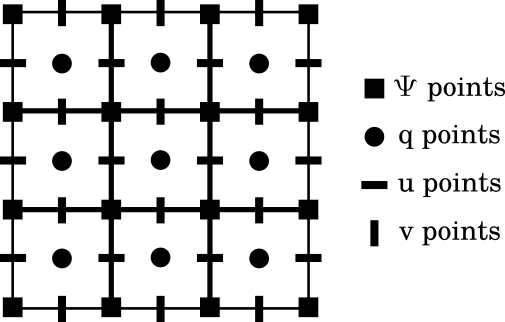
\includegraphics{figures/c-grid.png} %%% Update to svg
    \caption{Arakawa C-Grid.}
    \label{fig:c-grid}
\end{figure}


In this work, we consider finite volume approximations to the Laplacian operators on the Arakawa C-grid. There are $N_x$ tracer cells in the x-direction and $N_y$ tracer cells in the y-direction ($q$ points in Figure \ref{fig:c-grid}). There are $(N_x+1) \times (N_y+1)$ stream-function/vorticity points ($\Psi$ points in Figure \ref{fig:c-grid}). The Dirichlet modes are defined on the $\Psi$ points, while the Neumann modes are defined on the $q$ (tracer) points. To handle irregular geometry, a mask is applied on the $\Psi$ point for the Dirichlet modes. In this arrangement, homogeneous Dirichlet boundary conditions are enforced on the $\Psi$ points on the grid boundary and at masked points for the Dirichlet modes. For the Neumann modes, Neumann boundary conditions are applied to the $u$ and $v$ points on the numerical grid boundary and at $u$ and $v$ points that lie between two masked $\Psi$ points. In a finite volume formulation, homogeneous Neumann boundary conditions on the boundaries of the tracer cells that abut irregular boundaries.

Next, we define the discretization of each of the eigenmode problems. Notationally, we define a grid function $f$ For relating tracer, $u$, $v$, $Psi$, and $q$ points, we define tracer cell $(i,j)$ has 
\begin{itemize}
    \item $u_{i,j}$ on the western face of the tracer cell
    \item $u_{i+1,j}$ on the eastern face of the tracer cell
    \item $v_{i,j}$ on the southern face of the tracer cell
    \item $v_{i,j+1}$ on the northern face of the tracer cell
    \item $\Psi_{i,j}$ on the south-western corner of the tracer cell
\end{itemize}
We use the difference operators
\begin{subequations}
    \begin{align}
        \delta_i: \delta_if &= f_{i+1/2,j}-f_{i-1/2,j} \\
        \delta_j: \delta_jf &= f_{i,j+1/2}-f_{i,j-1/2}
    \end{align}
\end{subequations}
the averaging operators
\begin{subequations}
    \begin{align}
        \bar{}^{i}: \bar{f}^{i} &= \frac{1}{2}(f_{i+1/2,j}+f_{i-1/2,j}) \\
        \bar{}^j: \bar{f}^{j} &= \frac{1}{2}(f_{i,j+1/2}+f_{i,j-1/2})
    \end{align}
\end{subequations}
and the discrete derivative operators
\begin{subequations}
    \begin{align}
        \delta_x: \delta_xf &= \frac{1}{\Delta x} \delta_i f \\
        \delta_y: \delta_yf &= \frac{1}{\Delta y} \delta_j f 
    \end{align}
\end{subequations}
A superscript on the $\delta_x$ or $\delta_y$ operator indicates the type of point on an Arakawa C-grid the input function starts as. For example, $\delta_x^c f$ indicates that $f$ is defined on the tracer points, while $\delta_x^\zeta f$ would indicate that $f$ is defined on the vorticity points.

Shifting an index by $1/2$ references the a different type of point on an Arakawa C-grid. For example, $(i+1/2,j)$ relative to $(i,j)$ at a $u$ grid point corresponds to tracer grid point $(i,j)$. Similarly $(i-1/2,j)$ relative to $(i,j)$ at a $u$ grid point corresponds to tracer grid point $(i-1,j)$.

Using this framework and the \eqref{eq:velocity-decomposition}, we can define
\begin{subequations}
    \begin{align}
        u_{i,j} = \delta_x^c \chi - \delta_y^\zeta \Psi \\
        v_{i,j} = \delta_y^c \chi + \delta_x^\zeta \Psi
    \end{align}
\end{subequations}
This definition naturally places the $\chi$ at the tracer points and the $\Psi$ at vorticity points.

The vertical component of the relative vorticity is calculated as
\begin{equation}
    \zeta = \mathcal{A}_\zeta^{-1} \left[ \delta_i ( \Delta y_c v ) - \delta_j( \Delta x_c u ) \right]
\end{equation}
Since the curl of a gradient on a Arakawa C-grid is discretely zero, the relative vorticity is only related to the $\Psi$
\begin{equation}
    \zeta = \mathcal{A}_\zeta^{-1} \left[ \delta_i ( \Delta y_c \delta_x^\zeta \Psi ) + \delta_j( \Delta x_c \delta_y^\zeta \Psi ) \right] \label{eq:discrete-stream-function-laplacian}
\end{equation}
Equation \eqref{eq:discrete-stream-function-laplacian} defines the Laplacian operator that we use in the calculation of the eigenmodes; specifically, the eigenvalue problem is discretely defined as
\begin{equation}
    \mathcal{A}_\zeta^{-1} \left[ \delta_i ( \Delta y_c \delta_x^\zeta \Psi ) + \delta_j( \Delta x_c \delta_y^\zeta \Psi ) \right] = \lambda \Psi_{(i,j)} \label{eq:dirichlet-mode-equation}
\end{equation}
with homogeneous Dirichlet boundary conditions. Note that \eqref{eq:dirichlet-mode-equation} is collocated with the vorticity points on the Arakawa C-grid. 

The divergence of the horizontal flow on a Arakawa C-grid is
\begin{equation}
    \nabla \cdot \vec{u} = \mathcal{V}_c^{-1}\left[ \delta_i( \Delta y_g \Delta r_f h_w u) + \delta_j( \Delta x_g \Delta r_f h_s v) \right]
\end{equation}
Assuming that the divergence of a curl is discretely zero, the divergence is related to the velocity potential through
\begin{equation}
    \nabla \cdot \vec{u} = \mathcal{V}_c^{-1}\left[ \delta_i( \Delta y_g \Delta r_f h_w \delta_x \chi) + \delta_j( \Delta x_g \Delta r_f h_s \delta_y \chi) \right]
\end{equation}
The discrete eigenvalue problem for the velocity potential is then defined as
\begin{equation}
   \mathcal{V}_c^{-1}\left[ \delta_i( \Delta y_g \Delta r_f h_w \delta_x \chi) + \delta_j( \Delta x_g \Delta r_f h_s \delta_y \chi) \right] = \sigma \chi_{(i,j)} \label{eq:neumann-mode-equation}
\end{equation}
with homogeneous neumann boundary conditions. Note that \eqref{eq:neumann-mode-equation} is collocated with the tracer points of the Arakawa C-grid.


To find the eigenpairs for the Dirichlet and Neumann mode operators, we use the Scalable Library for Eigenvalue Problem Computations (SLEPc) \cite{Hernandez2005}. SLEPc provides a framework for computing eigenvalues and eigenvectors of large matrices on distributed memory compute platforms. For our problem, the matrices we are working with are sparse and symmetric matrices. When computing the spectra, full accounting of energy across all length scales requires knowledge of all of the eigenvectors and eigenvalues. This can be achieved using direct solvers in the Eigenwert Löser für Petaflop Anwendungen (ELPA; in English “Eigenvalue Solvers for Petaflop Applications”) \cite{Marek2014,Aukenthaler2011} solver with SLEPc. 

Although SLEPc can work with matrix-free operators, wherein a method for the matrix-action can be provided, we opt to construct sparse matrices in the compressed sparse row format using PETSc (). Using built-in sparse matrix formats with SLEPc allows us to easily take advantage of distributed memory parallelism in the SLEPc+ELPA eigenpair solver. MQGeometry implements subroutines for calculating the Laplacian operators, so sparse matrices for Laplacians in irregular geometry are not readily available. However, we can diagnose the sparse matrices by passing impulse functions to routines that implement the Laplacian and using the result to diagnose the entries of the sparse matrices representative of the discrete operators \eqref{eq:dirichlet-mode-equation} and \eqref{eq:neumann-mode-equation}. This method of operator diagnosis as a sparse matrix is identical to that used in studies that required capturing the transport operators in general circulation models \cite{schoonover2023}.

One concern with this methodology is in the substantial memory requirements for computing spectra. For problems with $N$ degrees of freedom, storage of the sparse matrices is $\mathcal{O}(N)$, and storage of all eigenvectors is $\mathcal{O}(N^2)$. Consider a grid with $100 \times 100$ ($10^4$) grid cells. Storing the matrix operators and the eigenvectors alone requires $3 \times 10^8$ floating point values of storage. At single precision, this requires 1.2 GB of memory. For a $500 \times 500$ grid, however, the memory storage requirement is near 750 GB. Using 


\section{Results}

\begin{figure}
    \centering
    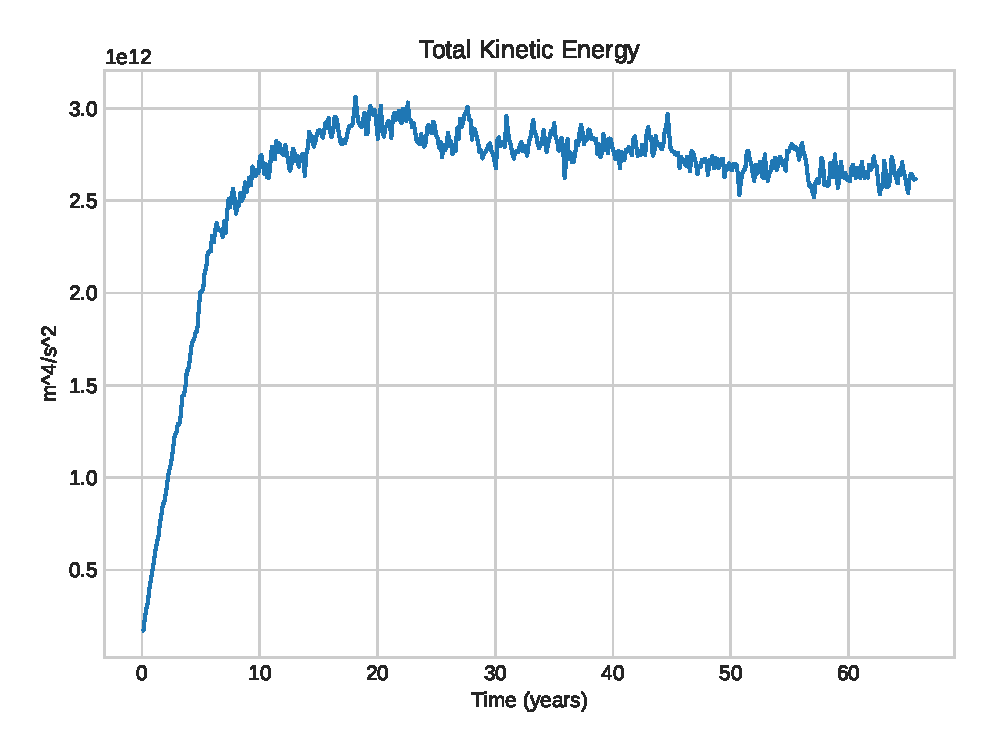
\includegraphics{figures/mqgeometry_cornercut/kinetic_energy_over_time.eps}
    
\includegraphics{figures/mqgeometry_dgirreg/kinetic_energy_over_time.eps}
    \caption{Kinetic energy over time for the upper layer of the three-layer quasi-geostrophic model. The left panel shows the corner cut domain, while the right panel shows the irregular domain.} \label{fig:kinetic-energy-over-time}
\end{figure}

\begin{figure}
    \centering
    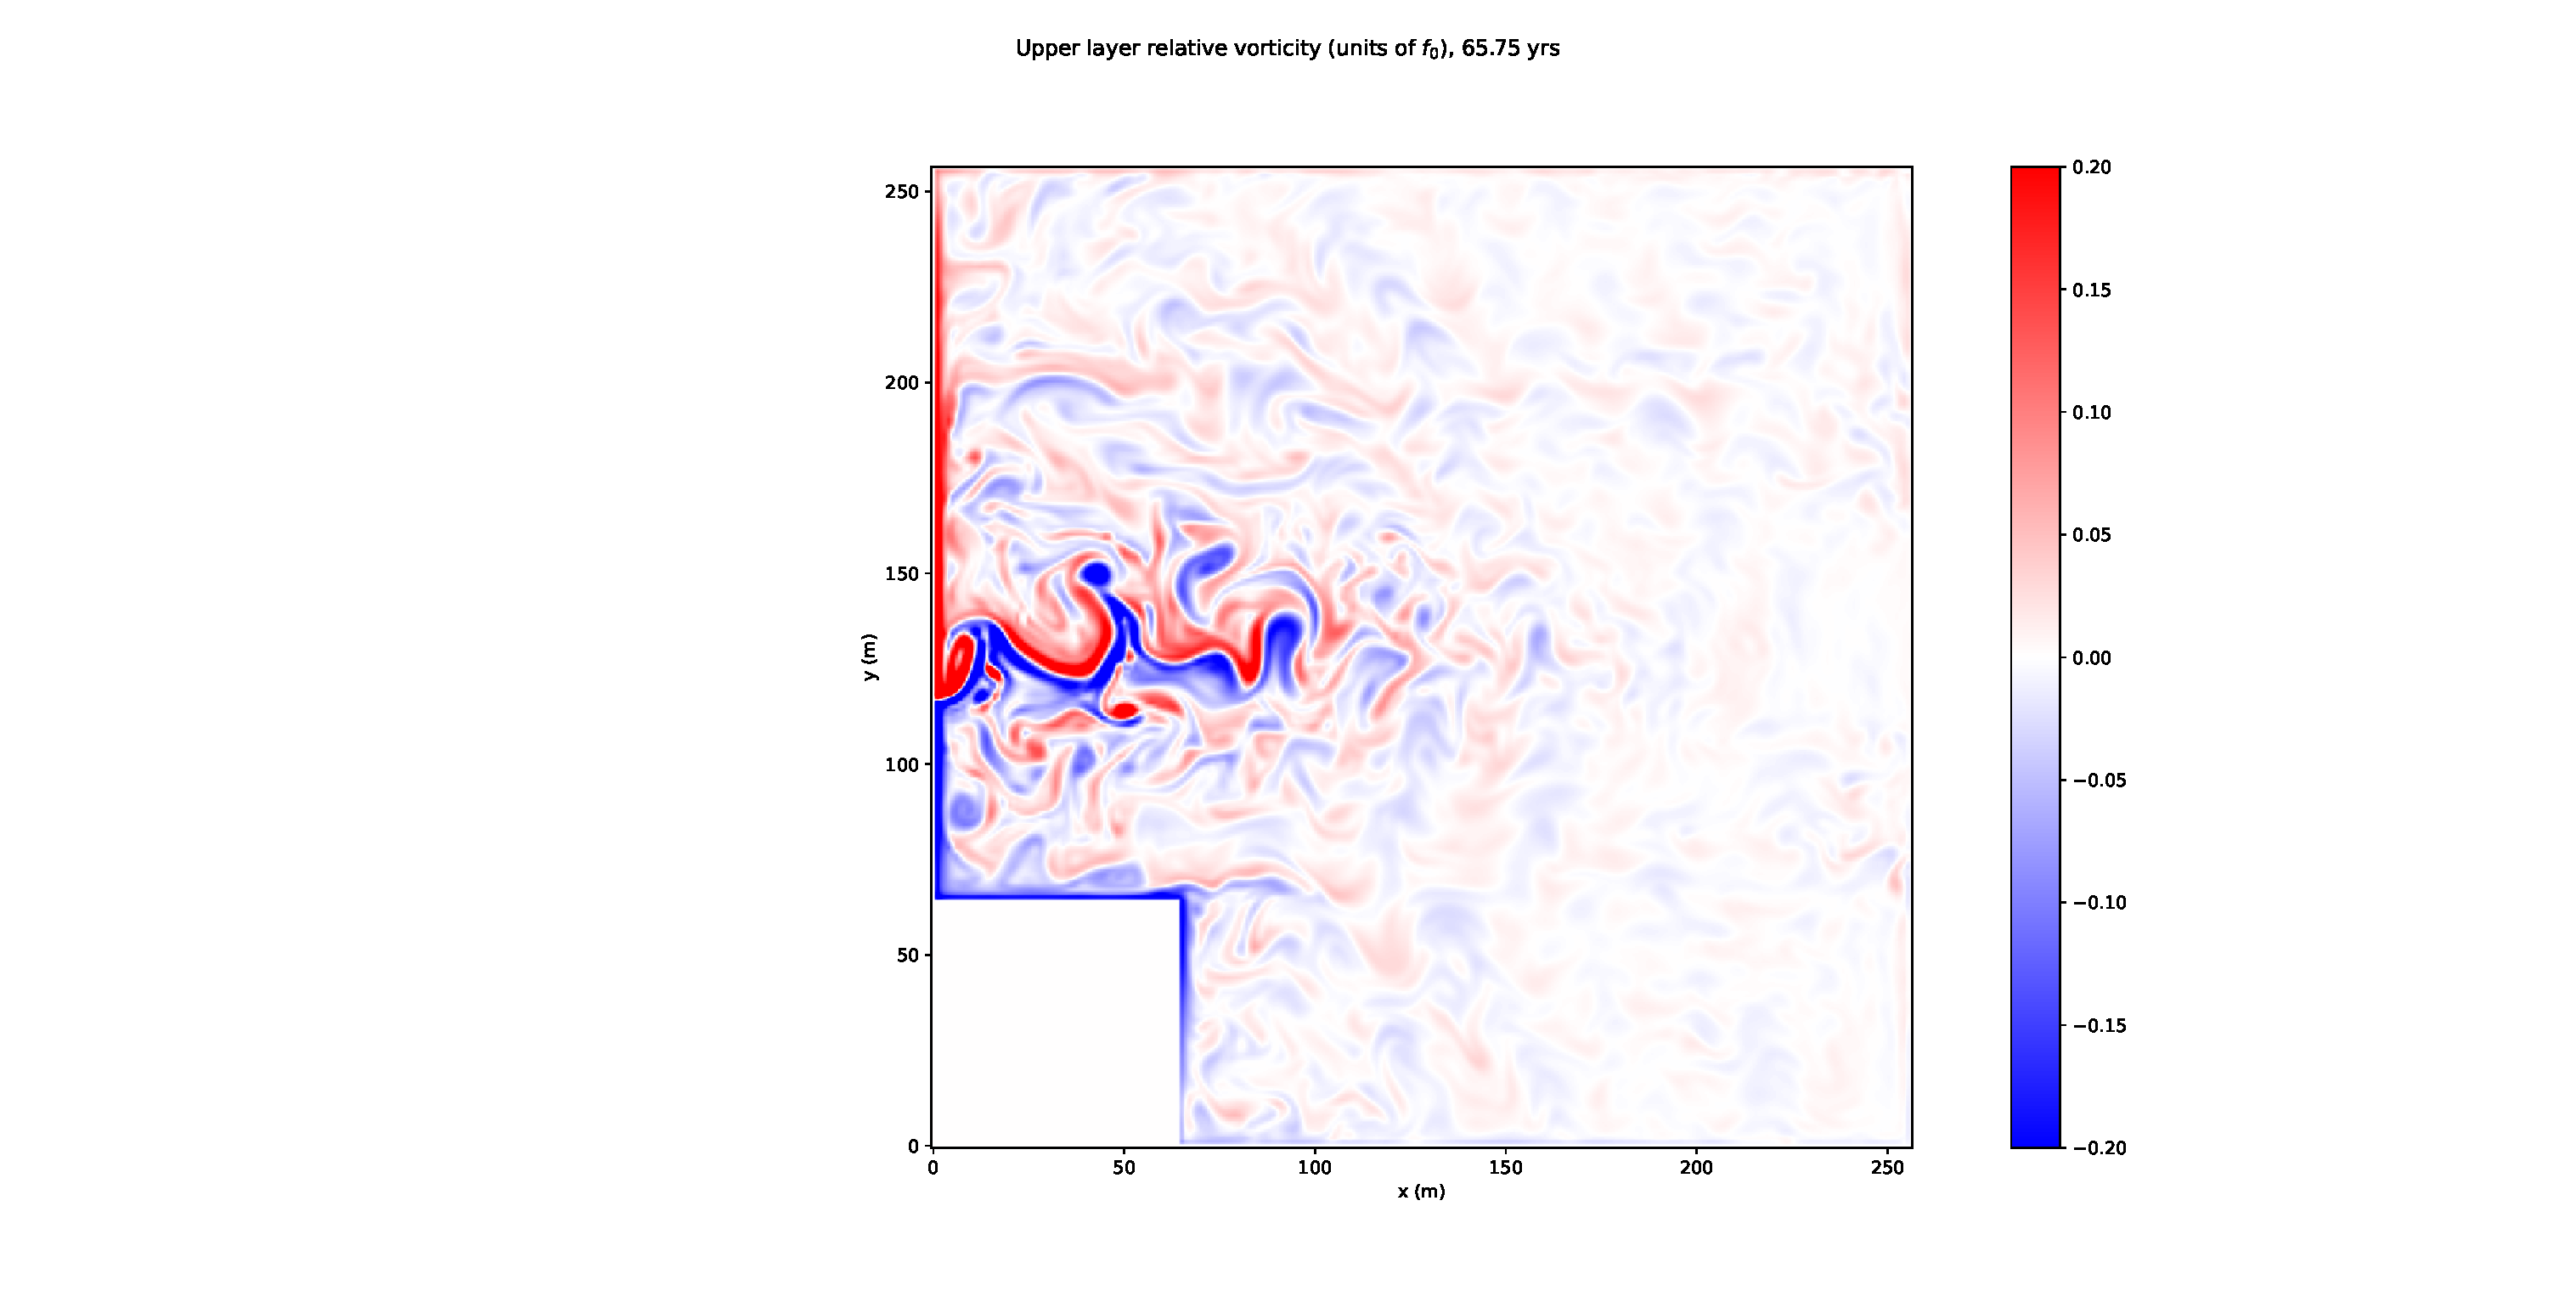
\includegraphics{figures/mqgeometry_cornercut/vort_518400.eps}
    
\includegraphics{figures/mqgeometry_dgirreg/vort_518400.eps}
    \caption{Relative vorticity for the upper layer after 65 years of simulation. The left panel shows the corner cut domain, while the right panel shows the irregular domain.} \label{fig:vorticity-65-years}
\end{figure}

\begin{figure}
    \centering
    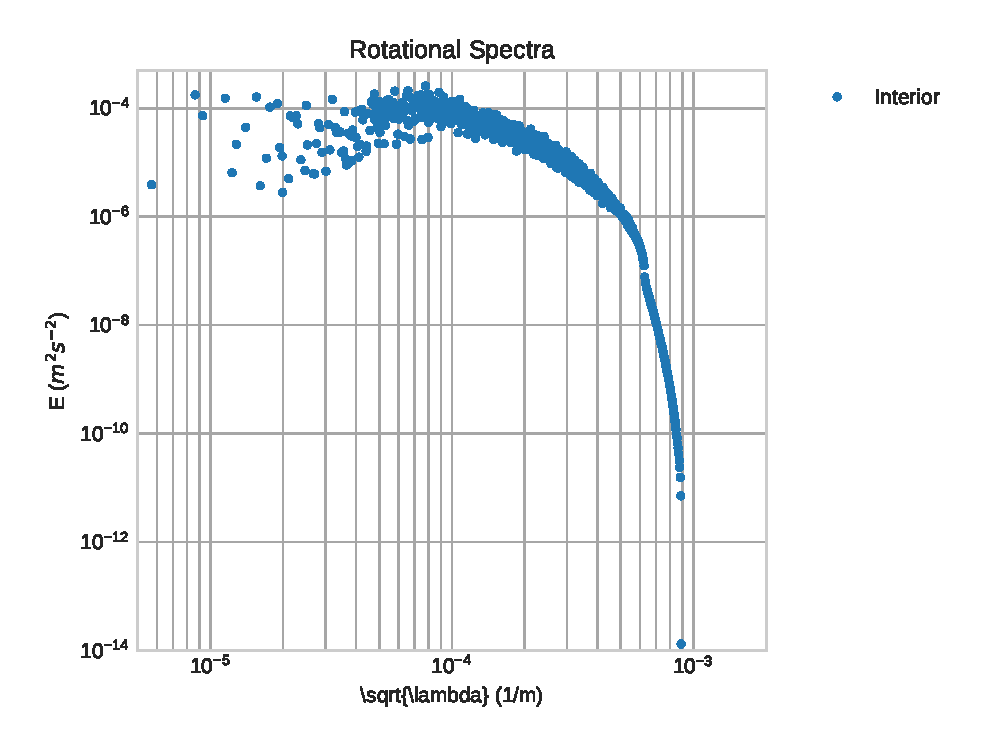
\includegraphics{figures/mqgeometry_cornercut/rotational_spectra.eps}
    
\includegraphics{figures/mqgeometry_dgirreg/rotational_spectra.eps}
    \caption{Rotational spectra for the upper layer of the three-layer quasi-geostrophic model. The left panel shows the corner cut domain, while the right panel shows the irregular domain. The spectra are computed after 100 years of simulation spinup.} \label{fig:rotational-spectra}
\end{figure}


\bibliography{name}


\end{document}
